\documentclass[xcolor=dvipsnames,compress]{beamer}
%\usepackage[latin1]{inputenc}
\usepackage{subfigure}
\usepackage{mpmulti}
\usepackage{epstopdf}

%
% Osnovna tema prosojnic je ULFRI
% Ce zelite uporabiti mini-frames temo (kot jo imata Berlin ali Warsaw) in jo radi uporabljajjo matematiki, 
% izberite \usetheme[compress]{ULFRIframes}
%
\usetheme[height=9mm]{ULFRI}
%\usetheme[compress]{ULFRIframes}

\title[FbHash]
{FbHash: shema za izra\v{c}un podobnosti datotek v digitalni forenziki}


\author[Knez, Mežnar, Pegan] % (optional, use only with lots of authors)
{Timotej Knez\inst{1},  Sebastian Mežnar\inst{2}, Jasmina Pegan\inst{1}}
% - Give the names in the same order as the appear in the paper.
% - Use the \inst{?} command only if the authors have different
%   affiliation.

\institute[UL FRI, UL FMF] % (optional, but mostly needed)
{
  \inst{1}%
  Fakulteta za računalništvo in informatiko\\
  Univerza v Ljubljana
  \and
  \inst{2}%
  Fakulteta za matematiko in fiziko\\
  Univerza v Ljubljana
}
% - Use the \inst command only if there are several affiliations.
% - Keep it simple, no one is interested in your street address.

\date[DigFor20] % (optional, should be abbreviation of conference name)
{}
% - Either use conference name or its abbreviation.
% - Not really informative to the audience, more for people (including
%   yourself) who are reading the slides online


%
% Ce uporabite mini-frames temo, potem vkljucite logo na naslovnici s spodnjim ukazom:
%
% logo of my university
%\titlegraphic{
\includegraphics[height=20mm]{znakULFRIbeamer.png}}


% If you wish to uncover everything in a step-wise fashion, uncomment
% the following command: 

%\beamerdefaultoverlayspecification{<+->}


\begin{document}

\begin{frame}
\titlepage
\end{frame}
%%%%%%%%%%%%%%%%%%%%%%%%%%%%%%%%%%%%%%%%%%%%%%%%%%%%%%%%%%%%%%%%%%%%%%%%%%%%%%%%
\section{Kazalo}
\label{sec:kazalo}
%%%%%%%%%%%%%%%%%%%%%%%%%%%%%%%%%%%%%%%%%%%%%%%%%%%%%%%%%%%%%%%%%%%%%%%%%%%%%%%%

\begin{frame}{Kazalo}
\begin{itemize}
  \item Uvod
  \item Sorodna dela
  \item Algoritem
  \item Eksperimenti v članku
  \item Naši eksperimenti
  \item Zaključek
\end{itemize}
\end{frame}


%%%%%%%%%%%%%%%%%%%%%%%%%%%%%%%%%%%%%%%%%%%%%%%%%%%%%%%%%%%%%%%%%%%%%%%%%%%%%%%%
\section{Uvod}
\label{sec:uvod}
%%%%%%%%%%%%%%%%%%%%%%%%%%%%%%%%%%%%%%%%%%%%%%%%%%%%%%%%%%%%%%%%%%%%%%%%%%%%%%%%

\begin{frame}{Uvod}
\begin{itemize}
	\item Avtomatizacija preiskave datotek
	\item Algoritmi za iskanje približnega ujemanja
	\begin{itemize}
		\item ssdeep, sdhash, FbHash
	\end{itemize}
	\item Prispevki članka
	\begin{itemize}
		\item odporna shema, dve različici, analiza varnosti
	\end{itemize}
	\item Implementacija algoritma
	\begin{itemize}
		\item različne funkcije za uteževanje
	\end{itemize}
	\item Testiranje na istih množicah kot v članku
\end{itemize}
\end{frame}



%%%%%%%%%%%%%%%%%%%%%%%%%%%%%%%%%%%%%%%%%%%%%%%%%%%%%%%%%%%%%%%%%%%%%%%%%%%%%%%%
\section{Sorodna dela}
\label{sec:sorodna}
%%%%%%%%%%%%%%%%%%%%%%%%%%%%%%%%%%%%%%%%%%%%%%%%%%%%%%%%%%%%%%%%%%%%%%%%%%%%%%%%

\begin{frame}{Sorodna dela}
\begin{itemize}
	\item ssdeep
	\begin{itemize}
		\item Temelji na algoritmu spamsum
		\item Funkcija z drsečim oknom
	\end{itemize}
	\item sdhash
	\begin{itemize}
		\item Statistično najmanj verjetni deli datoteke
		\item Bloomovi filtri
	\end{itemize}
	\item MRSH-v2
	\begin{itemize}
		\item Multi-resolution similarity hashing
		\item Funkcija z drsečim oknom, Bloomovi filtri
	\end{itemize}
	\item mvHash-B
	\begin{itemize}
		\item Krajšanje zapisa: glasovanje, kompakten zapis
		\item Bloomovi filtri
	\end{itemize}
\end{itemize}
\end{frame}
%

%%%%%%%%%%%%%%%%%%%%%%%%%%%%%%%%%%%%%%%%%%%%%%%%%%%%%%%%%%%%%%%%%%%%%%%%%%%%%%%%
\section{Algoritem}
%%%%%%%%%%%%%%%%%%%%%%%%%%%%%%%%%%%%%%%%%%%%%%%%%%%%%%%%%%%%%%%%%%%%%%%%%%%%%%%%

\begin{frame}{Algoritem}
\begin{itemize}
    \item An approximate multiplier, introduced by Babic et al. (2010):
    \item The product of the two numbers, $N_{1}$ and $N_{2}$ 
\end{itemize}
\end{frame}

%%%%%%%%%%%%%%%%%%%%%%%%%%%%%%%%%%%%%%%%%%%%%%%%%%%%%%%%%%%%%%%%%%%%%%%%%%%%%%%%
\section{Eksperimenti v članku}
\label{sec:eksoni}
%%%%%%%%%%%%%%%%%%%%%%%%%%%%%%%%%%%%%%%%%%%%%%%%%%%%%%%%%%%%%%%%%%%%%%%%%%%%%%%%

\begin{frame}{Eksperimenti v članku}
\begin{theorem}
  The probability of an error in the circuit is directly proportional
      to the trouble it can cause.
\end{theorem}
\pause
\begin{proof}
 The proof is straightforward.
\end{proof}
\end{frame}

%%%%%%%%%%%%%%%%%%%%%%%%%%%%%%%%%%%%%%%%%%%%%%%%%%%%%%%%%%%%%%%%%%%%%%%%%%%%%%%%
\section{Naši eksperimenti}
\label{sec:eksmi}
%%%%%%%%%%%%%%%%%%%%%%%%%%%%%%%%%%%%%%%%%%%%%%%%%%%%%%%%%%%%%%%%%%%%%%%%%%%%%%%%

\begin{frame}{Naši eksperimenti}
%
% --------------  Include the figures as follows -------------------%
%%
\begin{figure}[ht!]
    \label{fig:subfigures}
    \begin{center}
        \subfigure{%
            \label{fig:first}
            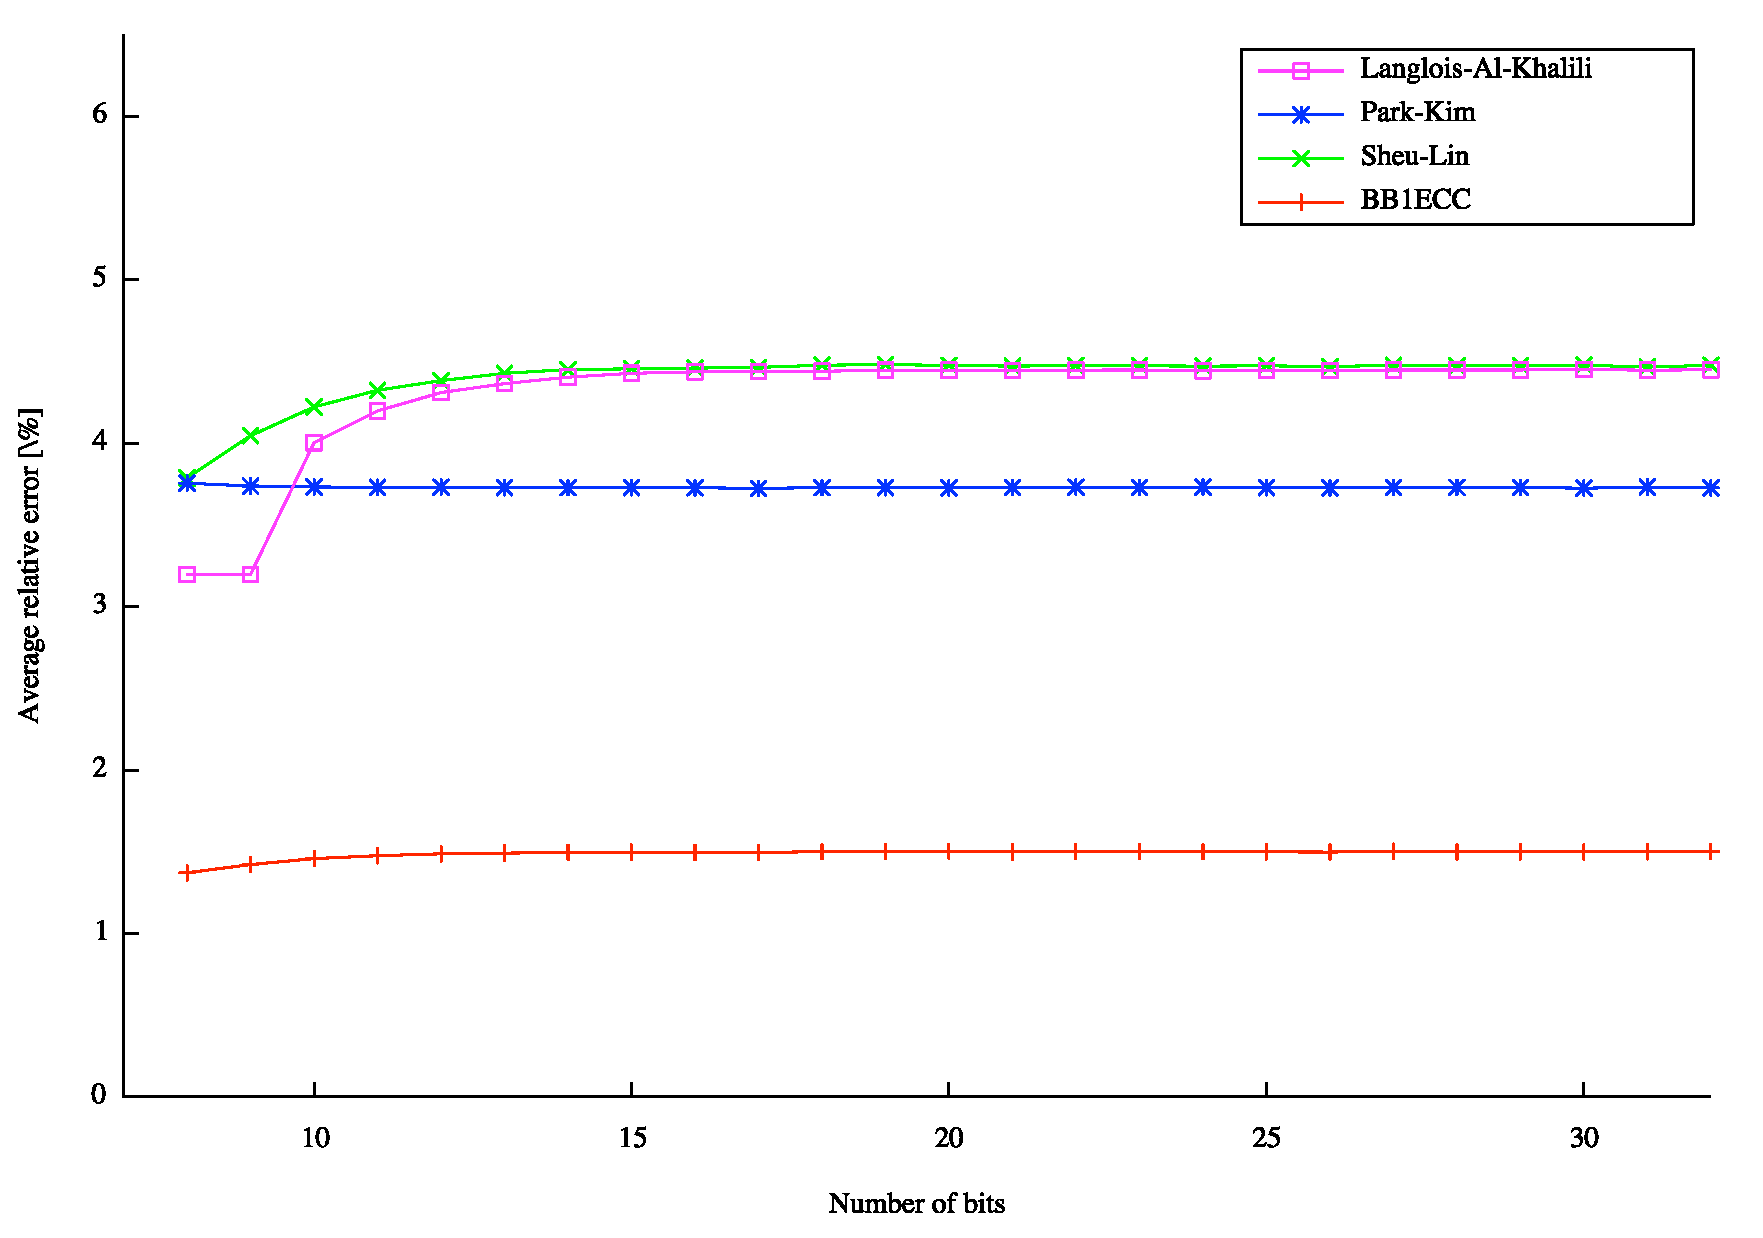
\includegraphics[width=0.4\textwidth]{figs/average.pdf}
        }%
        \subfigure{%
           %\label{fig:second}
           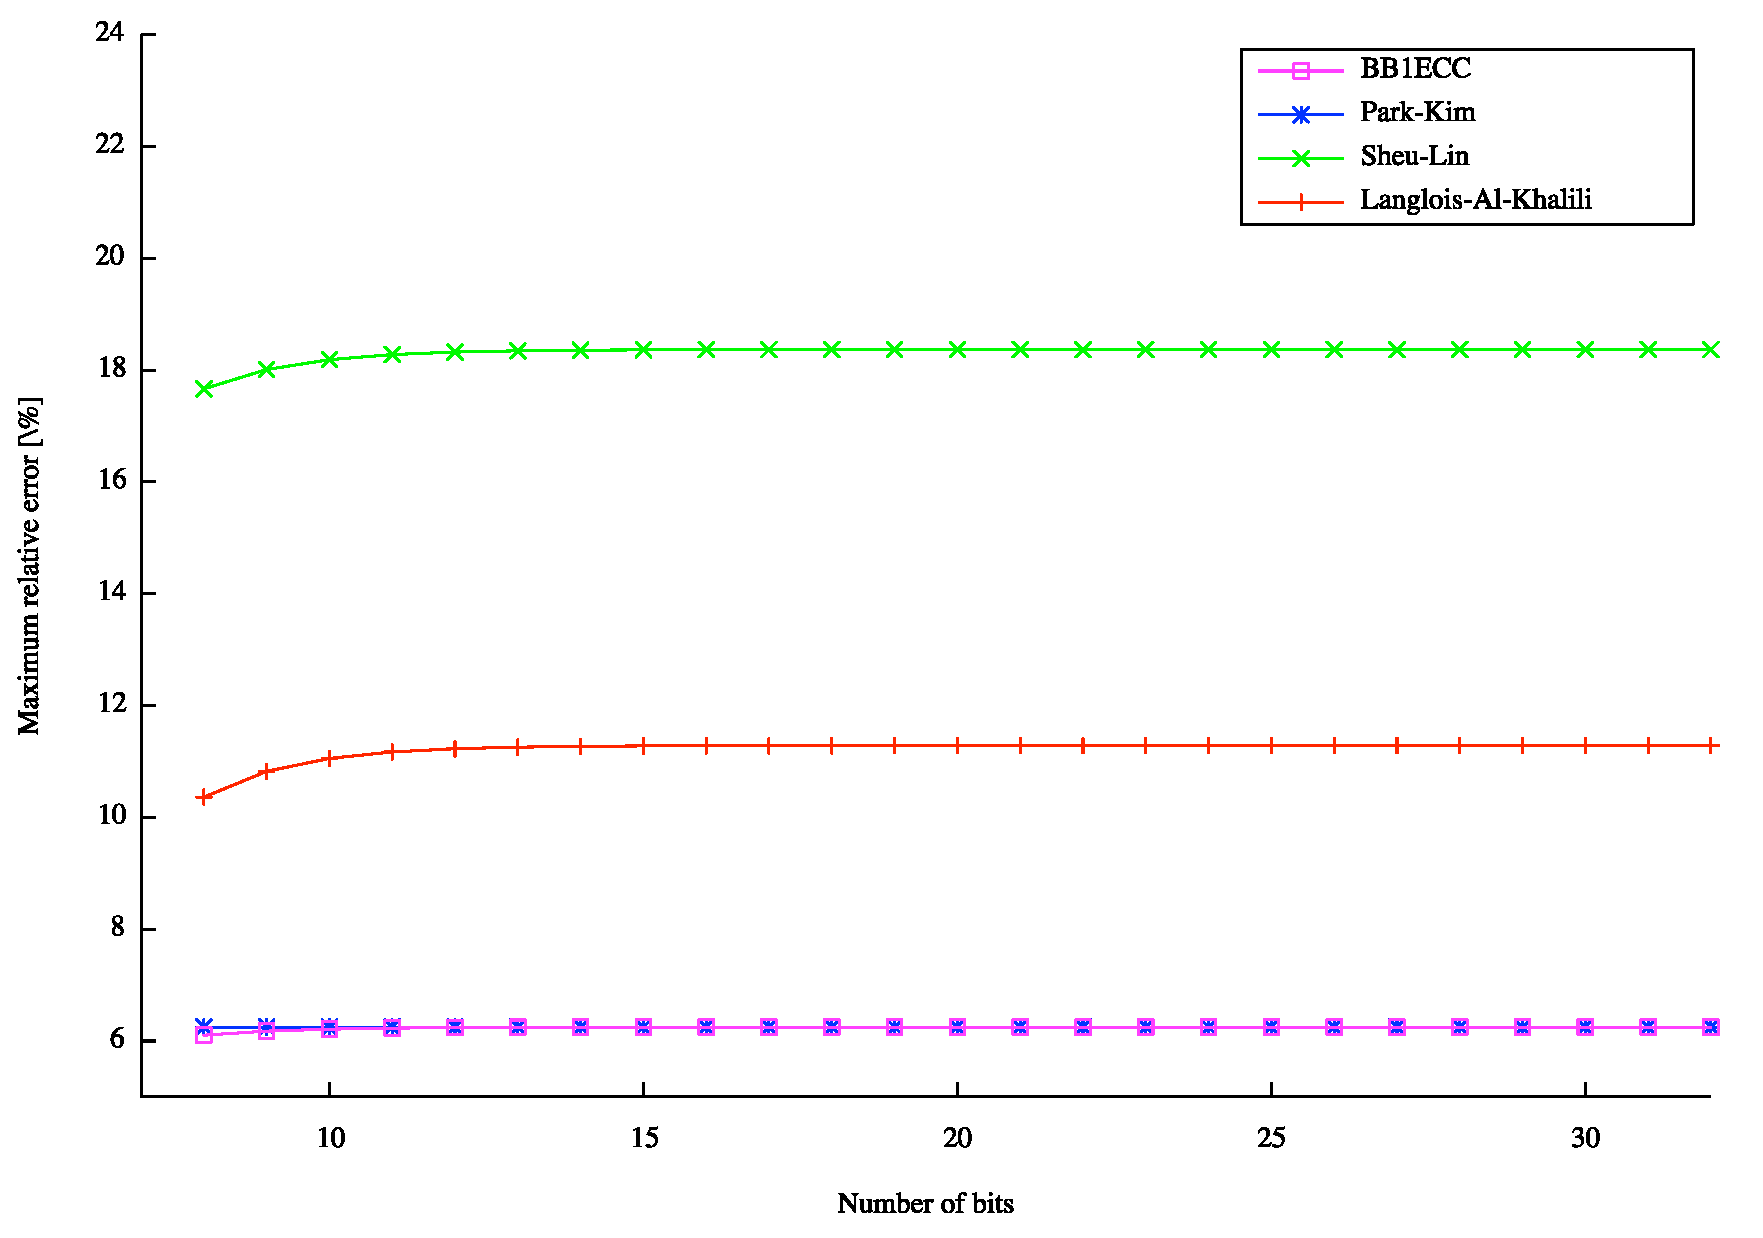
\includegraphics[width=0.4\textwidth]{figs/maximal.pdf}
        }\\ %  ------- End of the first row ----------------------%
        \subfigure{%
            \label{fig:third}
            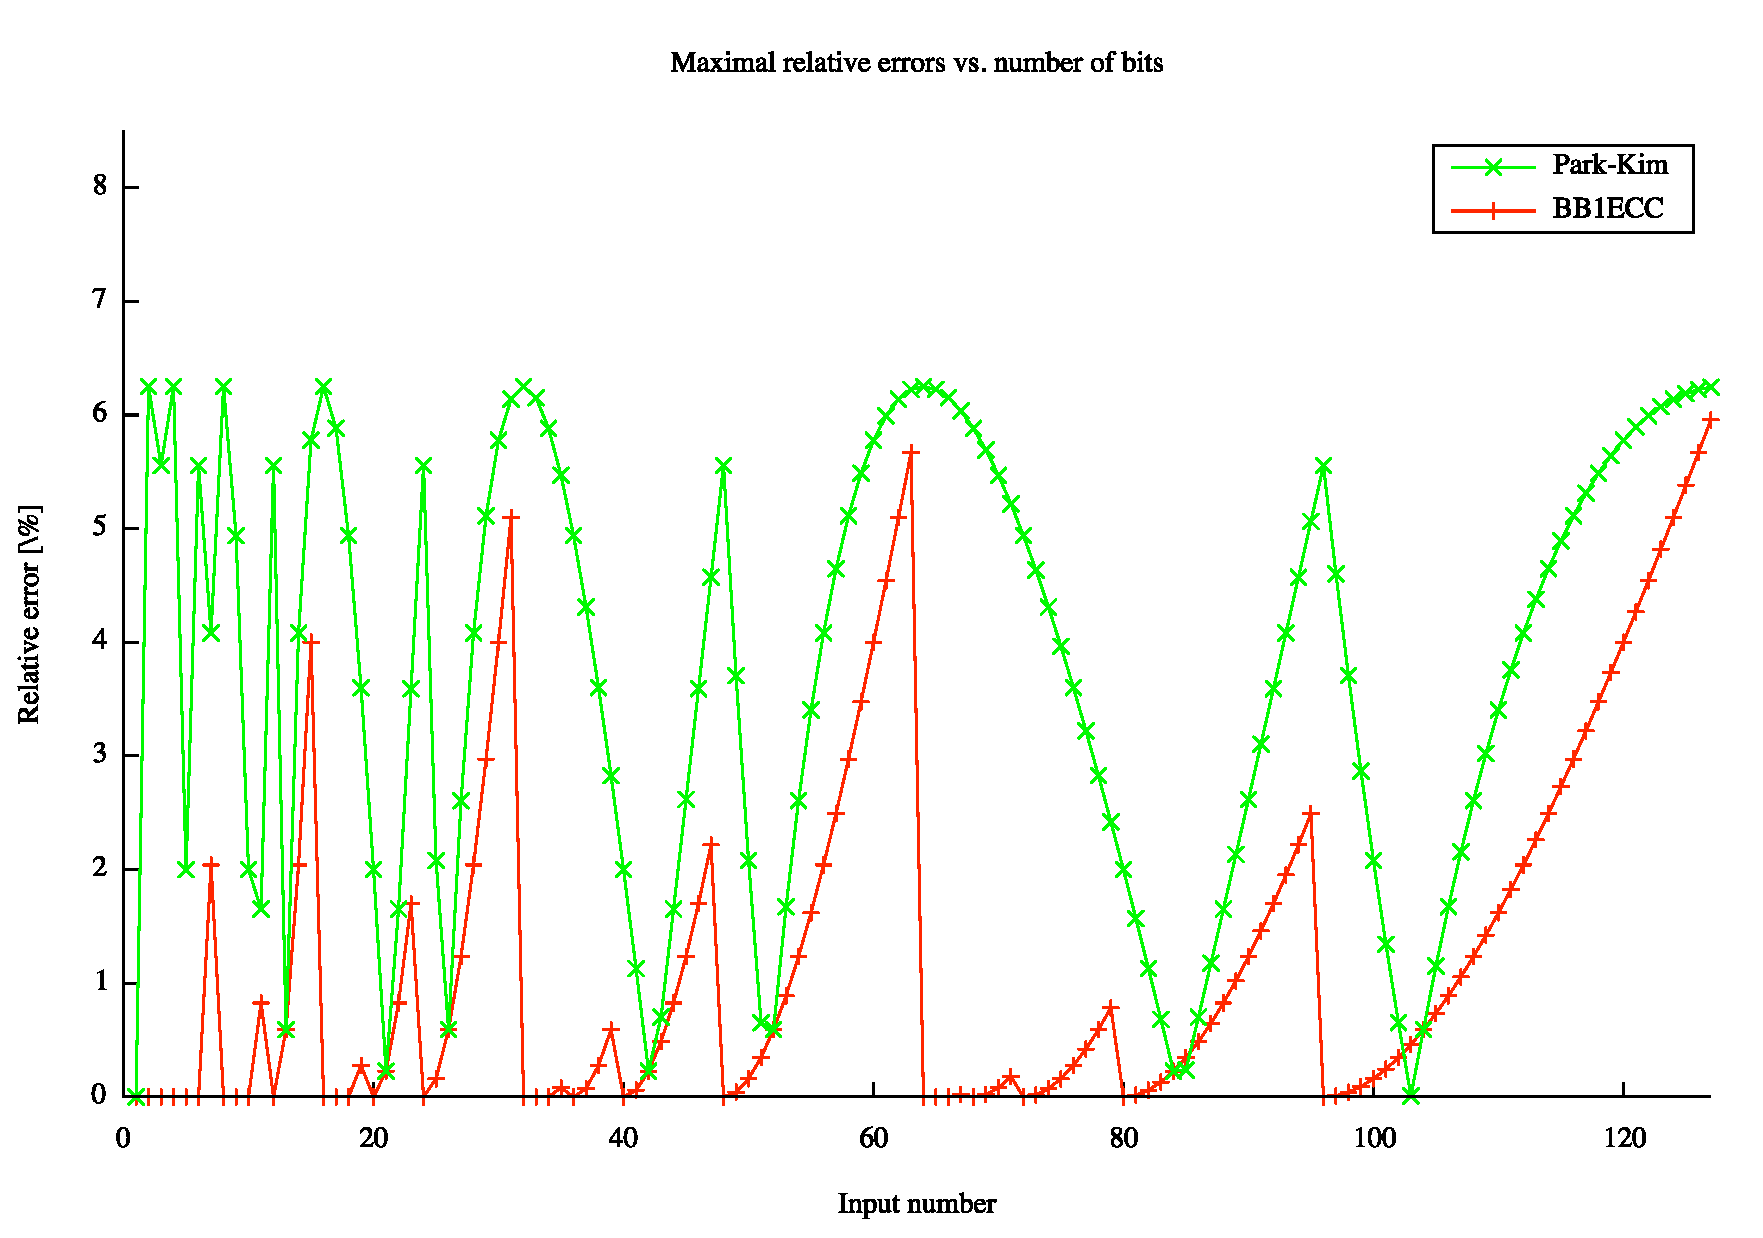
\includegraphics[width=0.4\textwidth]{figs/relative.pdf}
        }%
        \subfigure{%
            \label{fig:fourth}
            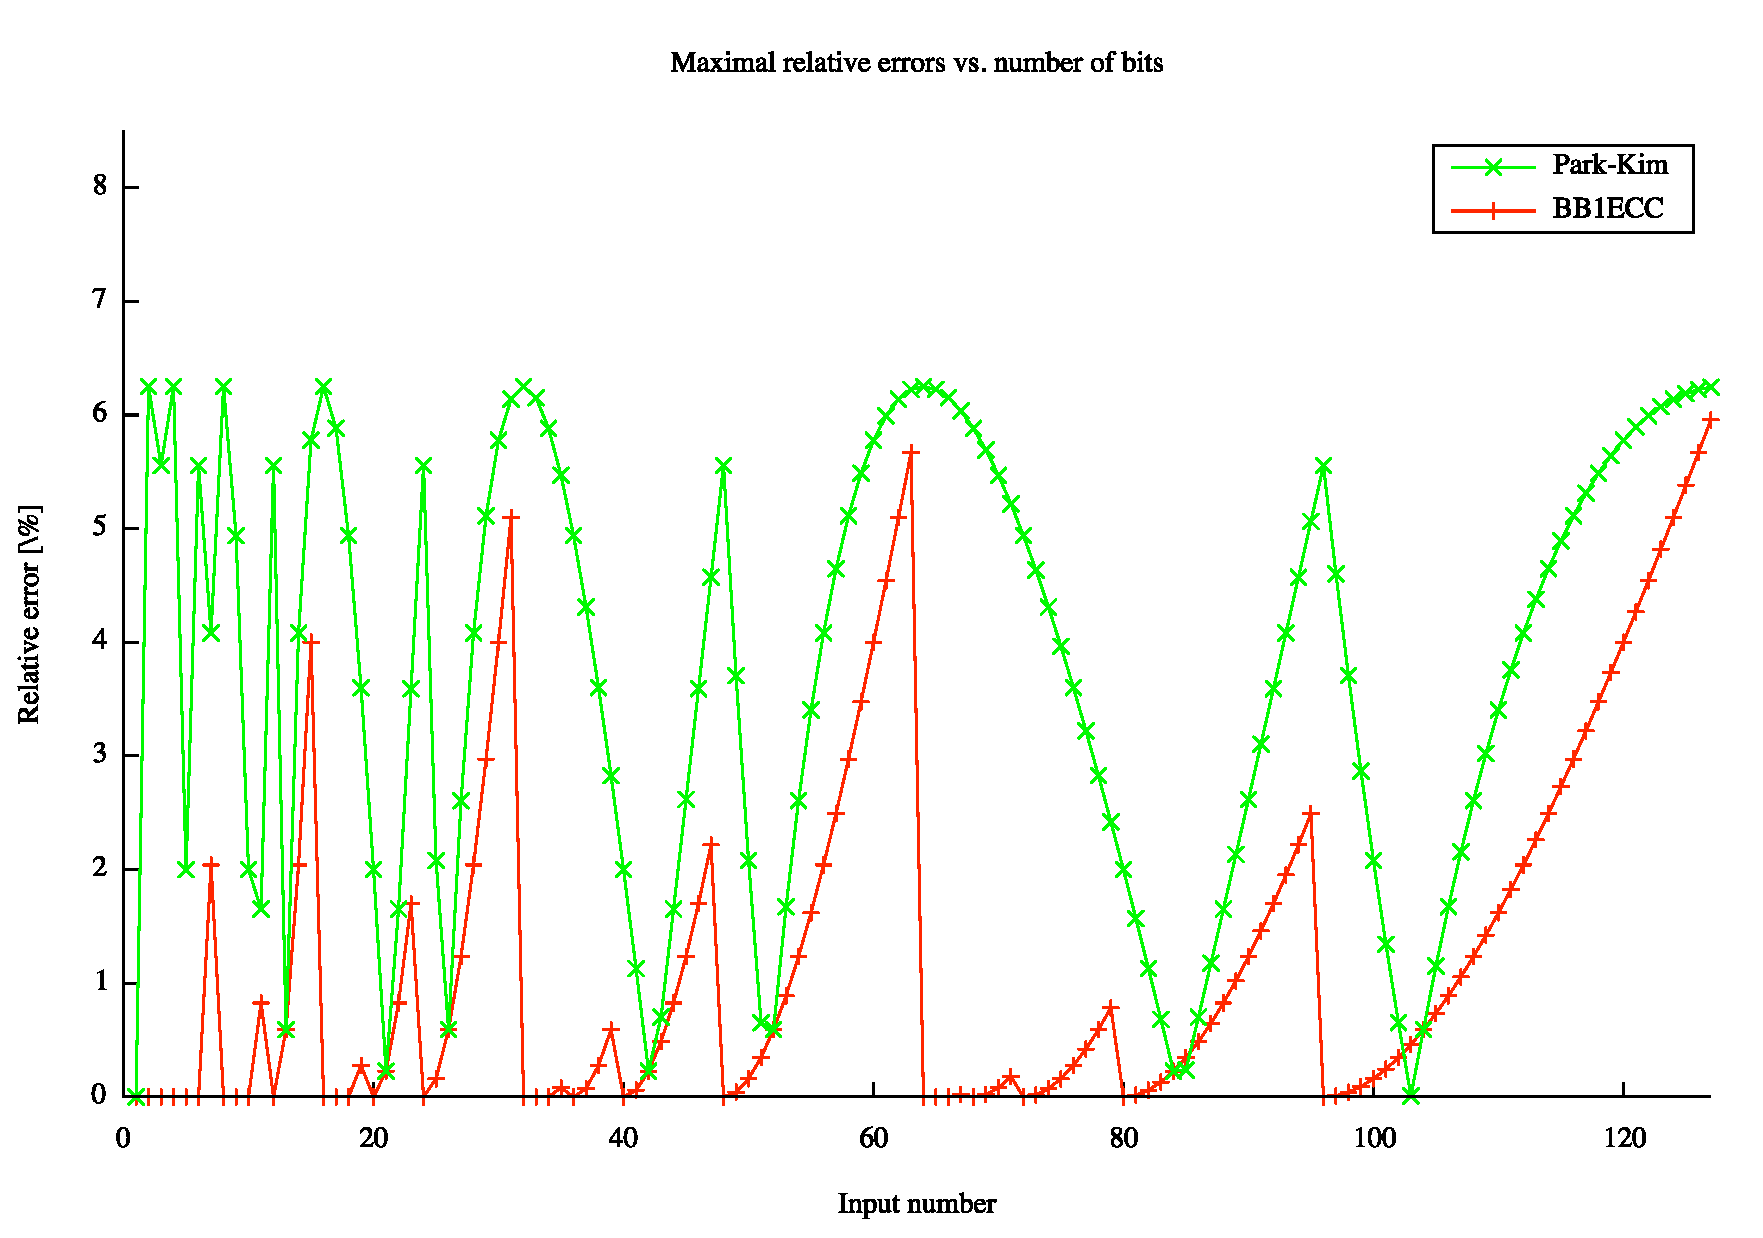
\includegraphics[width=0.4\textwidth]{figs/relative.pdf}
        }%
%
    \end{center}
   \caption{%
        The l-o-n-g caption for all the subfigures
        (FirstFigure through FourthFigure) goes here.
     }%
\end{figure}
%%
% -------------- End of figure environment ----------------------%
%%
\end{frame}






%%%%%%%%%%%%%%%%%%%%%%%%%%%%%%%%%%%%%%%%%%%%%%%%%%%%%%%%%%%%%%%%%%%%%%%%%%%%%%%%
\section{Zaključek}
\label{sec:zakljucek}
%%%%%%%%%%%%%%%%%%%%%%%%%%%%%%%%%%%%%%%%%%%%%%%%%%%%%%%%%%%%%%%%%%%%%%%%%%%%%%%%

\begin{frame}{Zaključek}
\begin{itemize}
	\item The proposed approach improves the average and maximum relative errors compared to the existing square approximations.
	\pause
	\item Error analysis has shown that an error in the circuit is directly proportional to the trouble it can cause.
\end{itemize}
\end{frame}



\end{document}